\documentclass[
  article,
  11pt,
  oneside,
  a4paper,
  english,
  brazil,
  sumario=tradicional
]{abntex2}

\usepackage{lmodern}
\usepackage[T1]{fontenc}
\usepackage[utf8]{inputenc}
\usepackage{indentfirst}
\usepackage{graphicx}
\usepackage{microtype}
\usepackage{amsmath}
\usepackage{booktabs}
\usepackage{tikz}
\usetikzlibrary{arrows.meta,fit,positioning}
\usepackage{pgfplots}
\pgfplotsset{compat=1.18,/pgf/number format/use comma}
\usepackage[alf]{abntex2cite}

\titulo{Segmentação de filamentos solares com U-Net e ResNet34: solução para o Desafio de Segmentação de Filamentos Solares 2026}
\tituloestrangeiro{Solar Filament Segmentation with U-Net and ResNet34}
\autor{Mauro Frank Lima de Lima\thanks{Pesquisador independente. Market Harborough, Reino Unido. E-mail: \texttt{mauro.frank.lima@outlook.com}.}}
\local{Brasil}
\data{2026}

\setlrmarginsandblock{3cm}{3cm}{*}
\setulmarginsandblock{3cm}{3cm}{*}
\checkandfixthelayout
\setlength{\parindent}{1.3cm}
\setlength{\parskip}{0.2cm}
\SingleSpacing

\begin{document}
\selectlanguage{brazil}
\frenchspacing
\maketitle

\begin{resumoumacoluna}
Este artigo apresenta a solução v13 para o Desafio de Segmentação de Filamentos Solares 2026, uma competição Kaggle sobre segmentação automática de filamentos solares em observações GONG de H-alfa. Treinamos uma U-Net com codificador ResNet34 em imagens MAGFiLO redimensionadas para $1024\times1024$ pixels, usando recortes aleatórios de $512\times512$, perda Dice e entropia cruzada binária ponderada (peso da classe positiva igual a 20). A inferência aplica uma única passagem por imagem, seguida de filtragem de componentes por probabilidade. O modelo v13 alcançou Dice de validação em recortes de 0,6275 e pontuação pública de 0,28. O arquivo CSV submetido contém 1.790 instâncias em 178 das 180 imagens de teste.

\vspace{\onelineskip}
\noindent
\textbf{Palavras-chave}: filamentos solares. H-alfa. U-Net. qualidade panóptica. MAGFiLO.
\end{resumoumacoluna}

\begin{center}\smaller
\textbf{Datas de submissão e aprovação}: não se aplica; este é um relatório técnico de competição, sem processo editorial.
\end{center}

\textual

\section{Introdução}

Este artigo descreve a solução submetida ao Desafio de Segmentação de Filamentos Solares 2026 \cite{filament-segmentation-2026}. A competição, lançada em 10 de julho de 2026, é organizada pelo laboratório Earth-Space AI Research (ESAIR)\footnote{\url{https://www.esairlab.com/home}}. A avaliação utiliza o conjunto de dados MAGFiLO \cite{ahmadzadeh2024dataset}.

Nossa abordagem converte um mapa de probabilidades de primeiro plano em instâncias individuais por meio de limiarização, fechamento morfológico e componentes conexos. A principal métrica da competição é a Qualidade Panóptica (PQ, do inglês \textit{Panoptic Quality}) \cite{kirillov2019panoptic}, definida por:
\begin{equation}
\mathrm{PQ} =
\frac{\sum_{(p,g)\in\mathrm{TP}} \mathrm{IoU}(p,g)}
{|\mathrm{TP}| + \tfrac{1}{2}|\mathrm{FP}| + \tfrac{1}{2}|\mathrm{FN}|},
\end{equation}
em que uma instância prevista $p$ é associada a uma instância de referência $g$ quando $\mathrm{IoU}(p,g)>0{,}5$. O avaliador exato é fornecido pelos organizadores da competição. Não foi medida a PQ de validação do modelo v13; o Dice em recortes apresentado neste trabalho é um diagnóstico distinto. O experimento v13 alterou a resolução de entrada, os recortes de treinamento, a ponderação da perda e a resolução de inferência em relação ao v12. Como essas alterações não foram avaliadas em ablações controladas, não é possível determinar a contribuição individual de cada uma.

\section{Metodologia}

\subsection{Visão geral do pipeline}

A Figura~\ref{fig:pipeline} apresenta o fluxo de dados completo, das imagens H-alfa originais de 2048 pixels às instâncias RLE submetidas.

\begin{figure}[htbp]
\centering
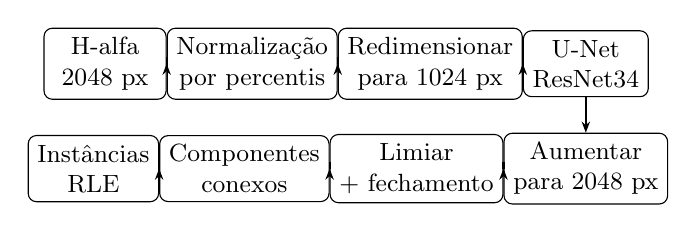
\begin{tikzpicture}[
  box/.style={draw, rounded corners=3pt, minimum width=1.55cm,
              minimum height=0.55cm, align=center, font=\small},
  arr/.style={-{Stealth[length=4pt]}, thick},
  node distance=0.22cm and 0.0cm
]
\node[box] (raw) {H-alfa\\2048 px};
\node[box, right=of raw] (norm) {Normalização\\por percentis};
\node[box, right=of norm] (res) {Redimensionar\\para 1024 px};
\node[box, right=of res] (unet) {U-Net\\ResNet34};
\node[box, below=0.45cm of unet] (up) {Aumentar\\para 2048 px};
\node[box, left=of up] (thr) {Limiar\\+ fechamento};
\node[box, left=of thr] (cc) {Componentes\\conexos};
\node[box, left=of cc] (rle) {Instâncias\\RLE};
\draw[arr] (raw) -- (norm);
\draw[arr] (norm) -- (res);
\draw[arr] (res) -- (unet);
\draw[arr] (unet) -- (up);
\draw[arr] (up) -- (thr);
\draw[arr] (thr) -- (cc);
\draw[arr] (cc) -- (rle);
\end{tikzpicture}
\caption{Pipeline de inferência de ponta a ponta. O treinamento usa o mesmo pré-processamento (metade esquerda), com recortes aleatórios de 512 pixels e aumento de dados.}
\label{fig:pipeline}
\par\smallskip{\footnotesize Fonte: elaboração própria.\par}
\end{figure}

\subsection{Dados e pré-processamento}

As imagens são arquivos JPEG em tons de cinza, com H-alfa e resolução de $2048\times2048$. O pré-processamento consiste em: (1) converter para tons de cinza; (2) normalizar as intensidades para o intervalo entre os percentis 1 e 99; e (3) redimensionar para $1024\times1024$. As máscaras de treinamento são rasterizadas a partir de anotações poligonais no formato COCO. A divisão do conjunto é feita por arquivo de imagem, na proporção 80/20 e com semente 0, resultando em 918 itens de treinamento e 236 de validação. A categoria 4 (Ambígua) é excluída; as três categorias restantes são combinadas em uma única classe de primeiro plano.

\subsection{Modelo e treinamento}

A arquitetura é \texttt{smp.Unet("resnet34", in\_channels=1)} \cite{ronneberger2015unet,he2016resnet}, com pesos do codificador pré-treinados no ImageNet.

A configuração de treinamento utiliza perda Dice (suavização igual a 1) combinada à entropia cruzada binária com \texttt{pos\_weight=20}; otimizador AdamW, taxa de aprendizado $\mathrm{lr}=5\times10^{-4}$, lote de tamanho 4 e 35 épocas. A taxa de aprendizado usa aquecimento de três épocas, seguido de decaimento cosseno. O aumento de dados aplica inversões horizontais e verticais aleatórias e rotações de 90 graus, sempre de forma conjunta à imagem e à máscara.

A combinação da perda Dice com entropia cruzada ponderada trata o desequilíbrio entre pixels de primeiro plano e de fundo nas imagens de filamentos: o termo Dice estabiliza o treinamento quando os pixels positivos são esparsos, enquanto \texttt{pos\_weight=20} amplifica o sinal de gradiente dos pixels de filamento. O ponto de verificação com o maior Dice de validação entre as 35 épocas foi selecionado. A Figura~\ref{fig:training} apresenta o Dice de validação por época.

\begin{figure}[htbp]
\centering
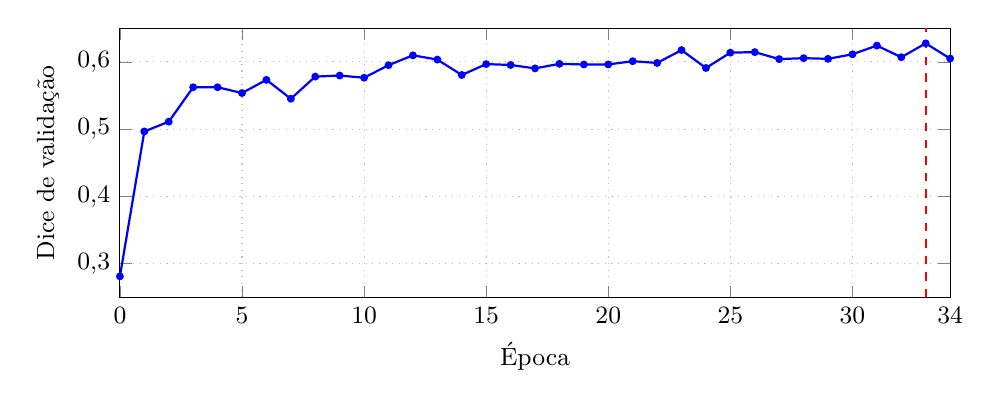
\begin{tikzpicture}
\begin{axis}[
  width=\textwidth, height=5cm,
  xlabel={Época}, ylabel={Dice de validação},
  xmin=0, xmax=34, ymin=0.25, ymax=0.65,
  xtick={0,5,10,15,20,25,30,34},
  ytick={0.3,0.4,0.5,0.6},
  grid=major, grid style={dotted},
  tick label style={font=\small},
  label style={font=\small},
  mark size=1pt
]
\addplot[blue, thick, mark=*] coordinates {
  (0,0.2813)(1,0.4966)(2,0.5111)(3,0.5623)(4,0.5623)
  (5,0.5537)(6,0.5733)(7,0.5452)(8,0.5781)(9,0.5797)
  (10,0.5764)(11,0.5951)(12,0.6097)(13,0.6034)(14,0.5805)
  (15,0.5967)(16,0.5954)(17,0.5903)(18,0.5971)(19,0.5961)
  (20,0.5962)(21,0.6010)(22,0.5984)(23,0.6175)(24,0.5909)
  (25,0.6137)(26,0.6145)(27,0.6041)(28,0.6055)(29,0.6045)
  (30,0.6113)(31,0.6242)(32,0.6069)(33,0.6275)(34,0.6049)
};
\addplot[red, dashed, thick] coordinates {(33,0.25)(33,0.65)};
\end{axis}
\end{tikzpicture}
\caption{Dice de validação por época. O melhor ponto de verificação foi obtido na época 33 (Dice = 0,6275; linha vermelha tracejada).}
\label{fig:training}
\par\smallskip{\footnotesize Fonte: registros do treinamento v13.\par}
\end{figure}

A Figura~\ref{fig:train-loss} apresenta a perda de treinamento registrada nas mesmas 35 épocas. O valor cai de 1,398 na época 0 para 0,421 na época 33 e sobe para 0,427 na época 34. Entre as épocas 25 e 34, o Dice de validação em recortes varia de 0,6041 a 0,6275, enquanto a perda de treinamento varia de 0,4206 a 0,4517. O valor da época 33 é o maior observado, mas esta série única, calculada em recortes, não demonstra que ele seja consistentemente superior aos valores das épocas próximas; não foram calculados intervalos de incerteza.

\begin{figure}[htbp]
\centering
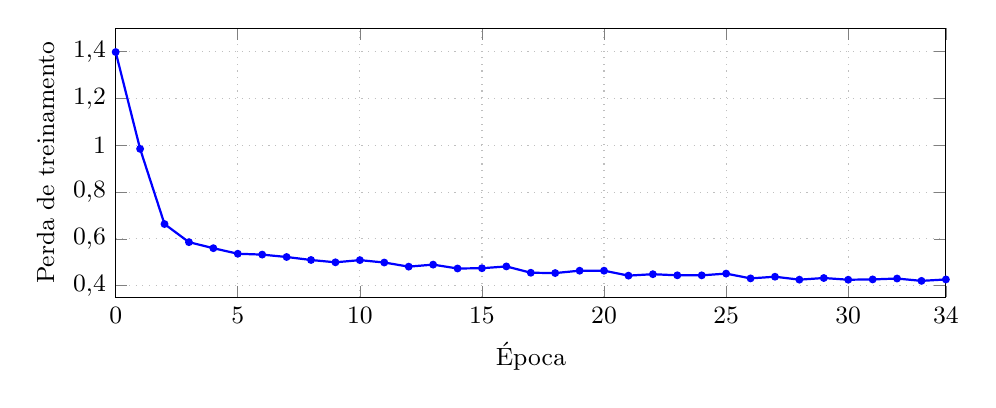
\begin{tikzpicture}
\begin{axis}[
  width=\textwidth, height=5cm,
  xlabel={Época}, ylabel={Perda de treinamento},
  xmin=0, xmax=34, ymin=0.35, ymax=1.5,
  xtick={0,5,10,15,20,25,30,34},
  ytick={0.4,0.6,0.8,1.0,1.2,1.4},
  grid=major, grid style={dotted},
  tick label style={font=\small},
  label style={font=\small},
  mark size=1pt
]
\addplot[blue, thick, mark=*] coordinates {
  (0,1.3983)(1,0.9846)(2,0.6634)(3,0.5860)(4,0.5602)
  (5,0.5365)(6,0.5328)(7,0.5226)(8,0.5098)(9,0.4999)
  (10,0.5092)(11,0.4990)(12,0.4814)(13,0.4900)(14,0.4735)
  (15,0.4746)(16,0.4823)(17,0.4553)(18,0.4540)(19,0.4641)
  (20,0.4641)(21,0.4430)(22,0.4491)(23,0.4444)(24,0.4442)
  (25,0.4517)(26,0.4312)(27,0.4383)(28,0.4258)(29,0.4328)
  (30,0.4255)(31,0.4268)(32,0.4306)(33,0.4206)(34,0.4267)
};
\end{axis}
\end{tikzpicture}
\caption{Perda de treinamento registrada em cada uma das 35 épocas.}
\label{fig:train-loss}
\par\smallskip{\footnotesize Fonte: registros do treinamento v13.\par}
\end{figure}

O Dice de validação é calculado com limiar de 0,5 em recortes aleatórios de 512 pixels das imagens de validação redimensionadas. Trata-se de um diagnóstico por recorte, não de uma métrica de imagem completa ou de instâncias.

\subsection{Inferência e pós-processamento}

Cada imagem de teste é redimensionada para $1024\times1024$ e processada em uma única passagem direta, sem aumento de dados em tempo de teste (TTA). O mapa de probabilidades é então ampliado para $2048\times2048$ por interpolação bilinear.

O pós-processamento tem quatro etapas. (1) Uma máscara-semente binária é formada com limiar $t_{\mathrm{lo}}=0{,}35$. (2) A máscara é fechada morfologicamente com um elemento estruturante elíptico de $5\times5$ para unir pequenas lacunas no interior dos filamentos. (3) São extraídos os componentes conexos da máscara fechada. (4) Cada componente é mantido como uma instância prevista se, e somente se, satisfizer os três critérios: probabilidade de pico $>t_{\mathrm{hi}}=0{,}50$, probabilidade média no componente $\geq\mathrm{min\_meanp}=0{,}30$ e área do componente $\geq\mathrm{min\_area}=50$ pixels \cite{afshar2026}. Todos os limiares são fixos para todas as imagens de teste; não há ajustes por imagem. Cada componente mantido é codificado como uma linha RLE (\textit{run-length encoding}) no CSV de submissão.

\section{Avaliação}

\begin{table}[htbp]
\centering
\caption{Configuração completa de treinamento e inferência do v13, obtida do campo \texttt{cfg} registrado em \texttt{train\_history.json}.}
\label{tab:cfg}
\begin{tabular}{ll}
\toprule
Parâmetro & Valor \\
\midrule
Codificador & resnet34 \\
Tamanho de entrada & $1024\times1024$ \\
Tamanho do recorte de treinamento & $512\times512$ \\
Tamanho do lote & 4 \\
Épocas & 35 \\
Taxa de aprendizado & $5\times10^{-4}$ \\
Fração de validação & 0,20 (semente 0) \\
\texttt{pos\_weight} & 20 \\
$t_{\mathrm{lo}}$ & 0,35 \\
$t_{\mathrm{hi}}$ & 0,50 \\
\texttt{min\_meanp} & 0,30 \\
\texttt{min\_area} & 50 px \\
Elemento de fechamento & elipse $5\times5$ \\
Tamanho de saída & $2048\times2048$ \\
\bottomrule
\end{tabular}
\par\smallskip{\footnotesize Fonte: configuração registrada no campo \texttt{cfg} de \texttt{train\_history.json}.\par}
\end{table}

\subsection{Resultados}

\begin{table}[htbp]
\centering
\caption{Resumo da submissão v13.}
\label{tab:results}
\begin{tabular}{lc}
\toprule
Quantidade & Valor \\
\midrule
Imagens de teste processadas & 180 \\
Imagens com previsões & 178 \\
Instâncias previstas & 1.790 \\
Instâncias por imagem, mediana (intervalo) & 10 (1--23) \\
Área RLE mínima & 50 px \\
Área RLE mediana & 1.014,5 px \\
Área RLE máxima & 25.043 px \\
TTA & Não \\
Resolução de treinamento & $1024\times1024$ (recorte $512\times512$) \\
Resolução de saída & $2048\times2048$ \\
Dice em recortes de validação (época 33) & 0,6275 \\
Pontuação pública na classificação & 0,28 \\
\bottomrule
\end{tabular}
\par\smallskip{\footnotesize Fonte: arquivo \texttt{submission\_v13.csv}.\par}
\end{table}

A Figura~\ref{fig:instance-counts} resume o número de instâncias mantidas por imagem de teste. As estatísticas de área da Tabela~\ref{tab:results} são calculadas a partir dos comprimentos de primeiro plano nas codificações RLE submetidas. Esses valores descrevem apenas a saída da submissão; sem anotações de teste, não medem a acurácia ou a completude da segmentação.

\begin{figure}[htbp]
\centering
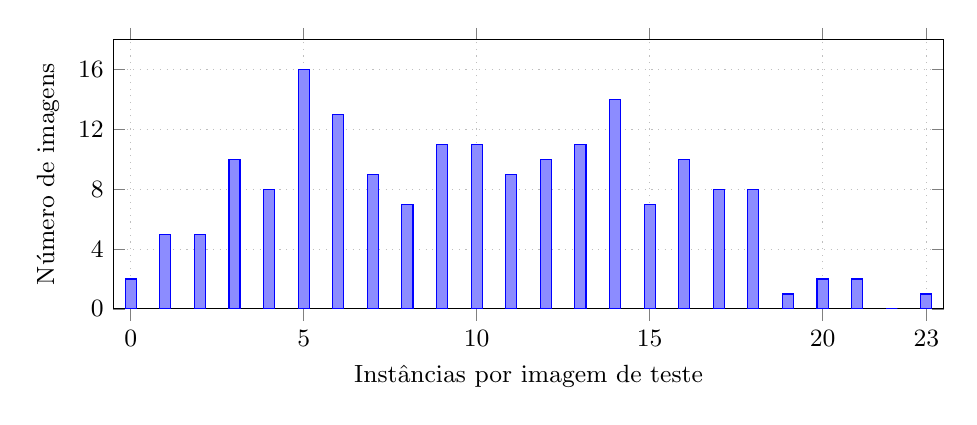
\begin{tikzpicture}
\begin{axis}[
  width=\textwidth, height=5cm,
  ybar, bar width=4pt,
  xlabel={Instâncias por imagem de teste},
  ylabel={Número de imagens},
  xmin=-0.5, xmax=23.5, ymin=0, ymax=18,
  xtick={0,5,10,15,20,23},
  ytick={0,4,8,12,16},
  grid=major, grid style={dotted},
  tick label style={font=\small},
  label style={font=\small},
]
\addplot[fill=blue!45, draw=blue] coordinates {
  (0,2)(1,5)(2,5)(3,10)(4,8)(5,16)(6,13)(7,9)
  (8,7)(9,11)(10,11)(11,9)(12,10)(13,11)(14,14)
  (15,7)(16,10)(17,8)(18,8)(19,1)(20,2)(21,2)(22,0)(23,1)
};
\end{axis}
\end{tikzpicture}
\caption{Instâncias RLE mantidas por imagem de teste nas 180 imagens; zero indica imagens sem linhas no CSV de submissão.}
\label{fig:instance-counts}
\par\smallskip{\footnotesize Fonte: arquivo \texttt{submission\_v13.csv}.\par}
\end{figure}

A submissão anterior v12 obteve pontuação 0,00, enquanto a v13 obteve 0,28 na classificação pública. O experimento v13 alterou várias configurações, incluindo resolução de entrada, recortes de treinamento, ponderação da perda e configuração de inferência. Essas alterações não foram testadas em ablações controladas; portanto, não é possível atribuir a melhora a uma alteração específica.

\subsection{Previsões qualitativas}

A Figura~\ref{fig:qualitative} apresenta três imagens de teste com diferentes números de instâncias. As cores distinguem as instâncias RLE; não há comparação com a referência real, pois as anotações das imagens de teste não estavam disponíveis.

\begin{figure}[htbp]
\centering
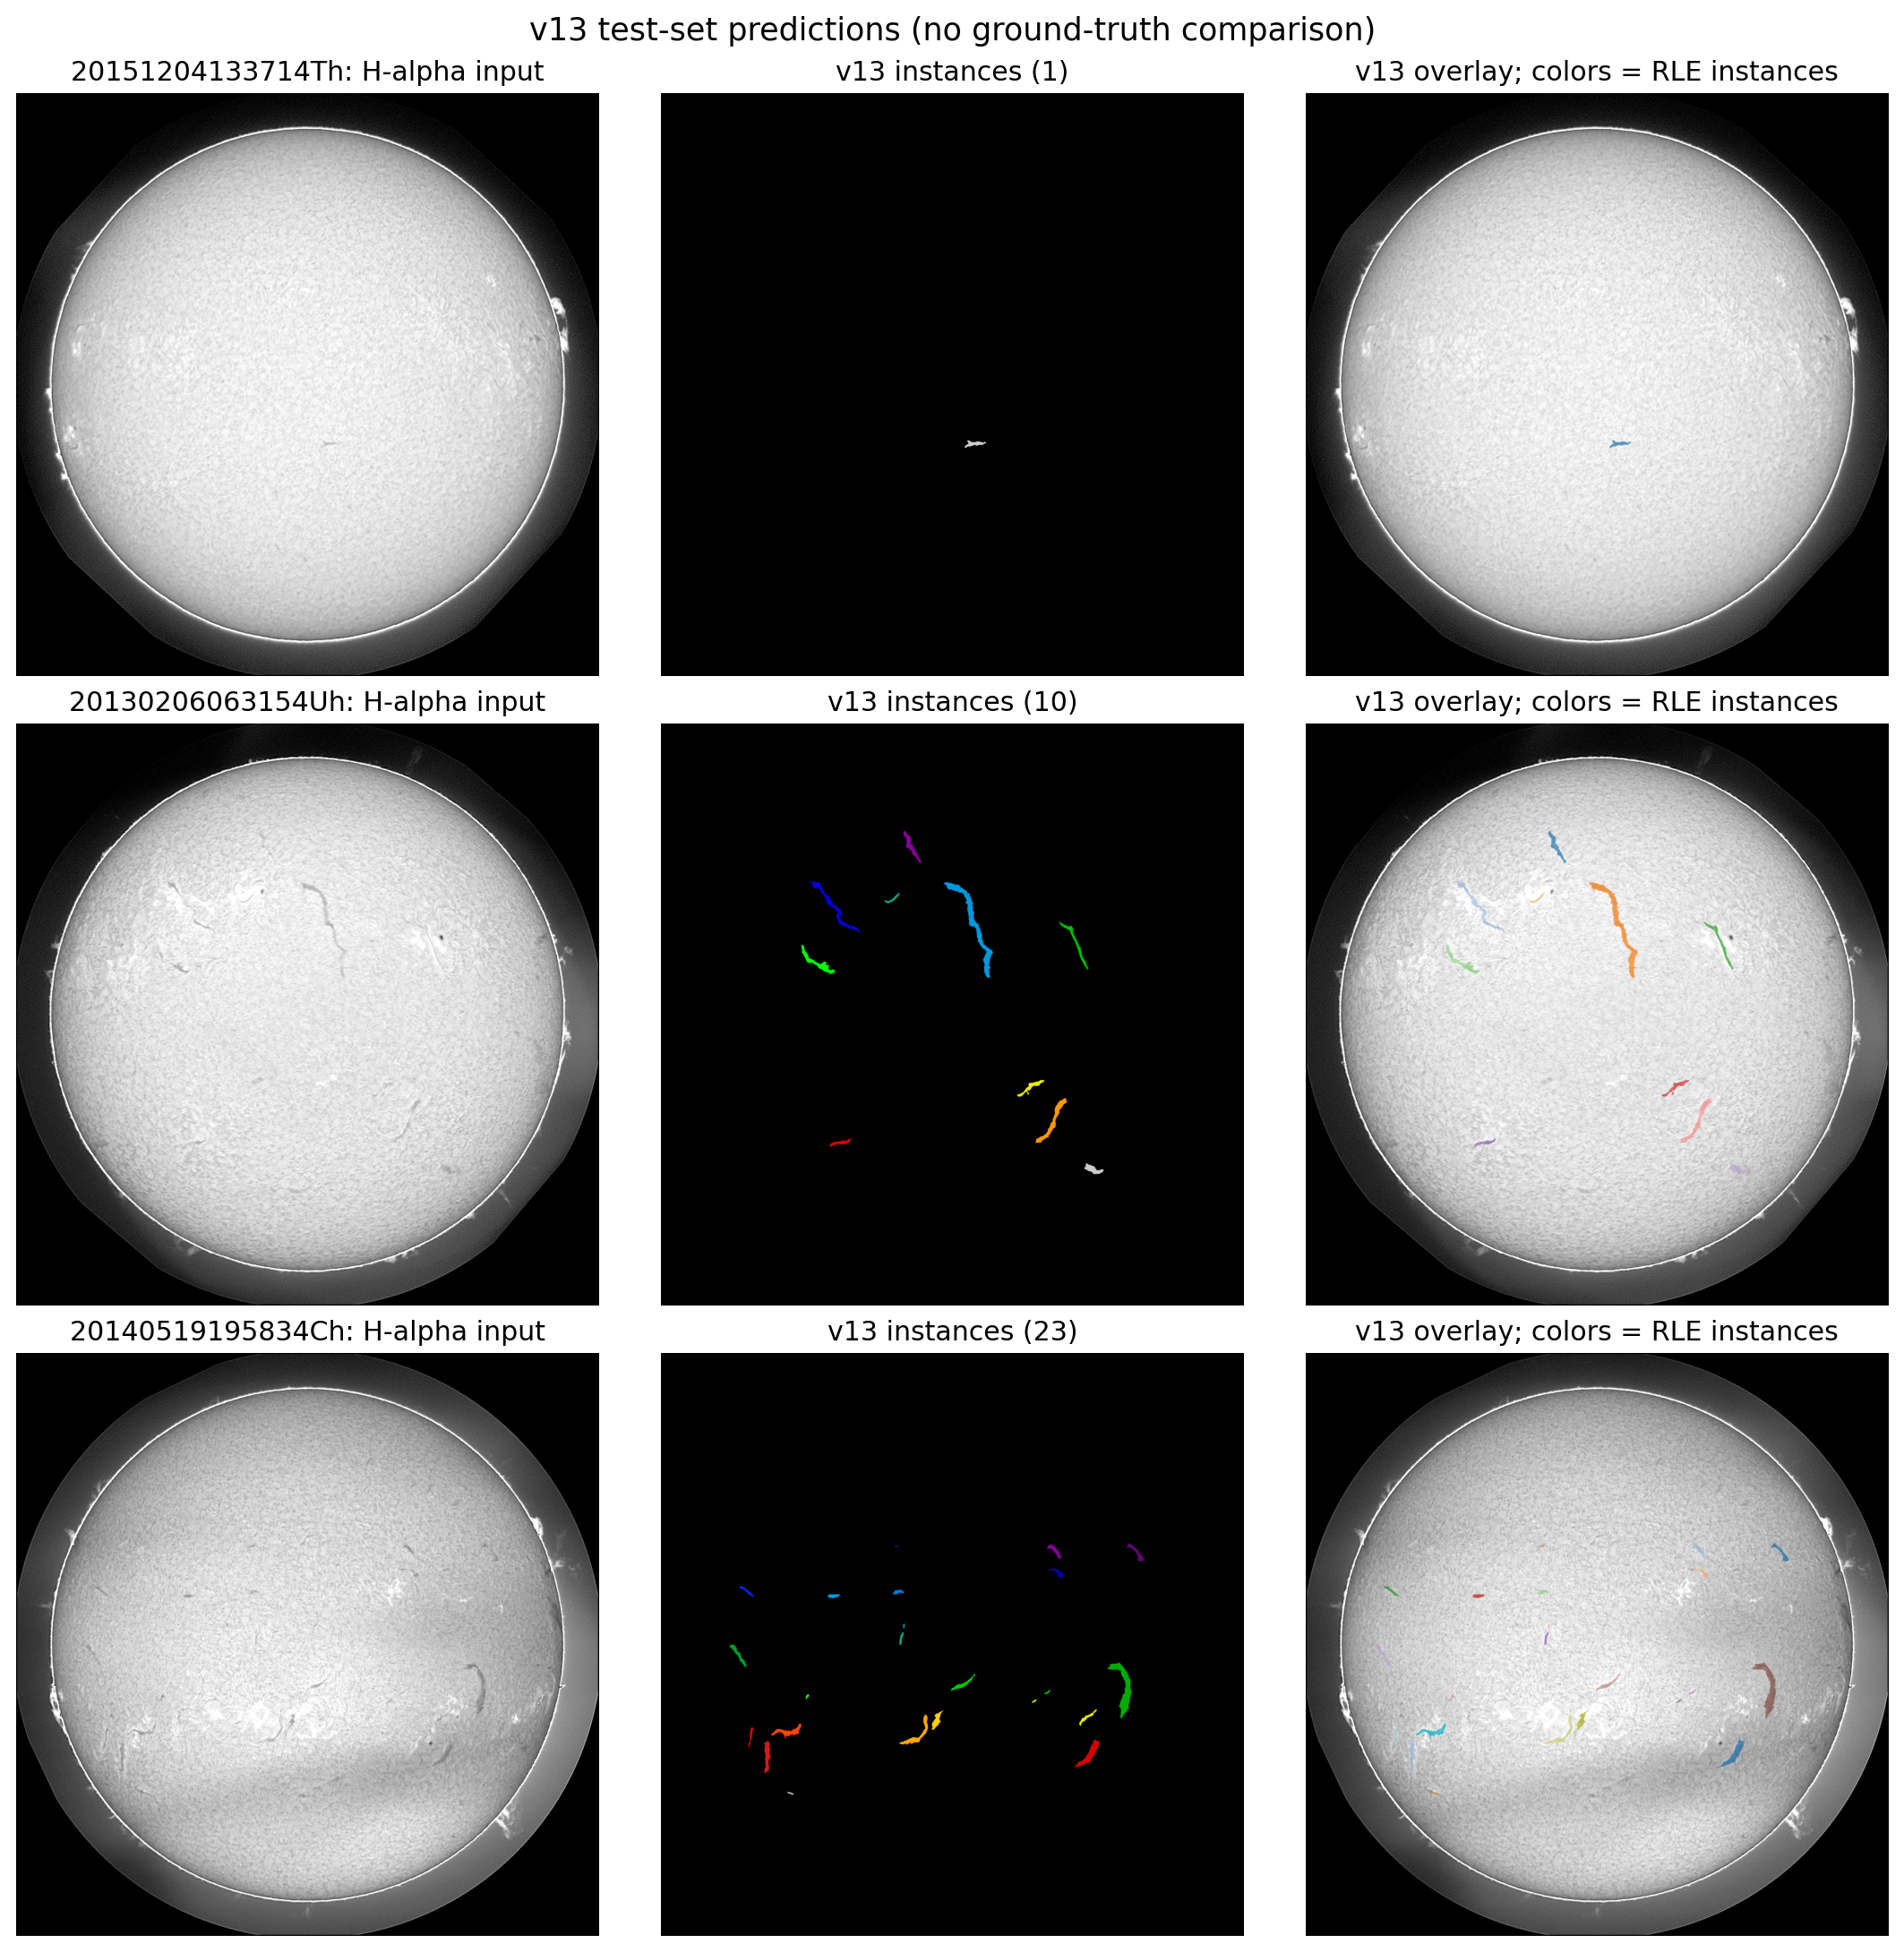
\includegraphics[width=0.9\textwidth]{v13_qualitative.png}
\caption{Previsões v13 nas imagens de teste 20151204133714Th (1 instância mantida), 20130206063154Uh (10) e 20140519195834Ch (23). Cada linha mostra a entrada H-alfa, as instâncias previstas e a sobreposição. As cores distinguem as instâncias. Não havia referência real disponível para o teste.}
\label{fig:qualitative}
\par\smallskip{\footnotesize Fonte: elaboração própria a partir das imagens de teste e das previsões do modelo v13.\par}
\end{figure}

\subsection{Pontos fortes, limitações e melhorias}

\textbf{Pontos fortes.} O pipeline é simples e reproduzível: usa limiares fixos, não aplica TTA e utiliza um único ponto de verificação. O codificador ResNet34 foi inicializado com pesos do ImageNet. A filtragem por componente (pico, média e área) tem como objetivo reduzir falsos positivos de regiões de baixa confiança sem exigir um classificador separado.

\textbf{Limitações.} Não foi medida a PQ de validação do v13; o Dice em recortes é uma métrica indireta que não otimiza diretamente o objetivo da competição. Duas imagens de teste não têm previsões; sem anotações de teste, não é possível determinar se isso representa falsos negativos ou imagens sem filamentos. O redimensionamento para 1024 pixels reduz detalhes espaciais de filamentos pequenos ou finos; os recortes aleatórios expõem o modelo a regiões locais, em vez de sempre ao contexto do disco solar completo. Os limiares fixos não foram selecionados por uma varredura de PQ concluída com os pesos v13. A combinação de três categorias de anotação em uma única classe de primeiro plano descarta distinções que podem ser relevantes para a avaliação.

\textbf{Melhorias.} A avaliação de PQ por instância em imagens completas de um conjunto de validação separado permitiria selecionar limiares de forma fundamentada. O aumento de dados em tempo de teste (inversão horizontal, inversão vertical e a combinação de ambas) é uma alternativa de baixo custo para melhorar a consistência dos contornos. Uma resolução de entrada maior, por exemplo, 2048 pixels de ponta a ponta, preservaria detalhes finos dos filamentos. Treinamento multiescala e inferência em blocos sobrepostos são próximos passos naturais. Uma ablação controlada, variando uma configuração por vez, ajudaria a esclarecer quais alterações influenciam a pontuação. Separar as três categorias de anotação em canais de saída distintos poderia melhorar a detecção e a classificação.

\subsection{Reprodutibilidade}

O código, o ponto de verificação (\texttt{weights/best.pt}) e o notebook de inferência (\texttt{pipeline.ipynb}) estão disponíveis em:
\begin{center}
\url{https://github.com/maurolima-sys/solar-filament-segmentation}
\end{center}
Para instalar as dependências, execute \texttt{pip install -r requirements.txt} e, em seguida, execute \texttt{pipeline.ipynb}. O notebook carrega \texttt{weights/best.pt} sem retreinamento e grava \texttt{submission\_v13.csv}. O CSV exato está incluído no repositório. A inferência pode ser executada em CPU ou GPU.

\section{Agradecimentos}

A organização do Desafio de Segmentação de Filamentos Solares 2026 recebe apoio parcial da Fundação Nacional de Ciência dos Estados Unidos (NSF), sob os auxílios n.º 2209912 e 2433781, da Diretoria de Ciência da Computação e Engenharia (CSE) e do Escritório de Ciberinfraestrutura Avançada (OAC), bem como do auxílio n.º 2511630, da Divisão de Ciências Astronômicas e da Diretoria de Ciências Matemáticas e Físicas (MPS).

O Desafio de Segmentação de Filamentos Solares 2026 é patrocinado pela NSF e pelo Observatório Solar Nacional dos Estados Unidos (NSO).

Este trabalho utiliza dados GONG obtidos pelo Programa Sinótico Integrado do NSO, administrado pelo Observatório Solar Nacional, operado pela Associação de Universidades para Pesquisa em Astronomia (AURA), Inc., sob acordo cooperativo com a NSF e com contribuições da Administração Nacional Oceânica e Atmosférica (NOAA). A rede GONG é hospedada pelo Observatório Solar Big Bear, pelo Observatório de Alta Altitude, pelo Observatório Solar de Learmonth, pelo Observatório Solar de Udaipur, pelo Instituto de Astrofísica das Canárias e pelo Observatório Interamericano de Cerro Tololo.

\postextual
\bibliographystyle{abntex2-alf}
\bibliography{referencias_ptbr}

\end{document}
